% ============================================================
%  IEEE-format report -- Brunner et al. (2012) Reproduction
%  Eranki Sai Vikas | Roll: 230121
%  Advanced Machine Learning -- Mid-Semester Examination Part B
% ============================================================
\documentclass[conference]{IEEEtran}

% ---- packages (hyperref MUST be last) --------------------------------
\usepackage[T1]{fontenc}
\usepackage[utf8]{inputenc}
\usepackage{amsmath,amssymb,amsfonts}
\usepackage{graphicx}
\usepackage{booktabs}
\usepackage{cite}
\usepackage{microtype}
\usepackage[caption=false,font=footnotesize]{subfig}
\usepackage[colorlinks=false,pdfborder={0 0 0}]{hyperref}

\graphicspath{{results/}}

% ---- title / author --------------------------------------------------
\title{Reproduction of ``Pairwise Support Vector Machines and their
Application to Large Scale Problems''}

\author{%
  \IEEEauthorblockN{Eranki Sai Vikas}
  \IEEEauthorblockA{Roll No: 230121 \\
    Advanced Machine Learning --- Mid-Semester Examination Part B \\
    Rishihood University, Sonipat, India \\
    \texttt{eranki.v23csai@nst.rishihood.edu.in}}
}

% ======================================================================
\begin{document}
\maketitle

% ----- Abstract --------------------------------------------------------
\begin{abstract}
We reproduce the core theoretical and empirical contribution of Brunner
et al.\ (2012)~\cite{brunner2012}: \emph{balanced pairwise kernels} for
Support Vector Machines, which enforce prediction symmetry for pair inputs
without doubling the training data. The Direct Linearised kernel $K_{DL}$
is implemented from scratch using \texttt{scikit-learn} on the Olivetti
Faces dataset. Two ablation studies isolate the role of (1)~the
symmetry-enforcing cross-terms and (2)~the feature dimensionality. A
failure-mode experiment reveals the method's brittleness under severe
pair-class imbalance. Results confirm the paper's central claim:
$K_{DL}$ consistently outperforms the non-symmetric baseline $K_D$ in
accuracy and AUC-ROC, and accuracy alone is a misleading metric under
imbalance.
\end{abstract}

\begin{IEEEkeywords}
Pairwise SVM, balanced kernels, face verification, ablation study,
kernel methods, reproducibility
\end{IEEEkeywords}

% ======================================================================
\section{Introduction and Paper Summary}

\textbf{Problem.}
Brunner et al.~\cite{brunner2012} address \textbf{pairwise classification}:
given two inputs $(a,b)$, decide whether they share the same class label.
The canonical application is face verification --- given two face images,
decide if they show the same person. Standard SVMs operate on single
inputs; extending them to input pairs requires careful treatment of
\emph{symmetry}: swapping $(a,b)$ to $(b,a)$ should not change the
prediction.

\textbf{Key contribution.}
The paper shows that two approaches to symmetry are \emph{theoretically
equivalent} (Theorem~3): (i)~doubling the training set by including every
pair in both orders, or (ii)~applying a \emph{balanced} pairwise kernel
on the original training set. The balanced approach is computationally
preferable since it avoids the $\times2$ data overhead.

\textbf{Experimental validation.}
On the Labeled Faces in the Wild (LFW) benchmark with hand-crafted
descriptors (SIFT, LBP, TPLBP), balanced kernels reduce the Equal Error
Rate (EER) from 0.0993 (plain $K_D$ baseline) to 0.0947 (balanced
$K_{DL}$), an improvement of $\sim$0.5 pp. While numerically modest, this
gap is consistent across all feature types and represents a measurable
advance over the state of the art at publication time.

% ======================================================================
\section{Method: Balanced Pairwise Kernels}

\subsection{Core Formulation}

Given inputs $a, b, c, d \in \mathcal{X}$ and a base Mercer kernel
$k: \mathcal{X}\times\mathcal{X}\to\mathbb{R}$, the plain
\emph{Direct Kernel} is:
\begin{equation}
  K_D\!\bigl((a,b),(c,d)\bigr) = k(a,c) + k(b,d)
  \label{eq:kd}
\end{equation}
Equation~\eqref{eq:kd} is \emph{not} symmetric in the pair argument ---
$K_D((a,b),(c,d)) \neq K_D((b,a),(c,d))$ in general. The paper's key
contribution, the \textbf{Direct Linearised Kernel}, adds cross-terms:
\begin{equation}
  K_{DL}\!\bigl((a,b),(c,d)\bigr)
    = \tfrac{1}{2}\bigl[k(a,c)+k(b,d)+k(a,d)+k(b,c)\bigr]
  \label{eq:kdl}
\end{equation}
Swapping $(a,b)\!\to\!(b,a)$ leaves~\eqref{eq:kdl} unchanged because
the $k(a,d)+k(b,c)$ terms simply switch roles (Theorem~2).
The $\tfrac{1}{2}$ factor normalises the scale relative to $K_D$.
A second family of kernels --- the \emph{Tanimoto Linearised} ($K_{TL}$)
and \emph{Mixed} ($K_{TM}$) variants --- apply the same idea to
ratio-based similarities and achieve the best empirical results in the
paper, but $K_{DL}$ is the focus of this reproduction because it is the
simplest case that illustrates the core idea.

\subsection{Theoretical Result (Theorem 3)}

The central theorem states: training an SVM with a \emph{symmetric}
training set $\hat{S}$ (every pair duplicated in both orders) using $K_D$
yields \emph{exactly} the same decision function as training with the
original set $S$ using $K_{DL}$. This equivalence means we never need to
physically double the dataset --- we only need to switch the kernel.

\subsection{Step-by-Step Pipeline}

\begin{enumerate}
  \item \textbf{Pair construction.} Build a binary dataset from all
        same-identity and different-identity image pairs. Label same-person
        pairs $+1$ and different-person pairs $-1$.
  \item \textbf{Feature extraction.} Apply PCA ($d=50$) to raw pixel
        vectors to obtain compact representations. The paper used
        SIFT/LBP/TPLBP; we use PCA due to hardware constraints.
  \item \textbf{Base kernel.} Compute the $n\!\times\!n$ RBF matrix
        $k(x_i,x_j)=\exp\!\left(-\gamma\|x_i-x_j\|^2\right)$ once and
        cache for reuse.
  \item \textbf{Pairwise kernel.} Assemble the
        $|\mathcal{P}|\!\times\!|\mathcal{P}|$ gram matrix $K_{DL}$ for
        all training pairs using cached base-kernel values.
  \item \textbf{SVM training.} Solve the soft-margin QP
        via \texttt{SVC(kernel="precomputed", C=1.0)}.
  \item \textbf{Prediction.} Output $\operatorname{sign}\!(\sum_i \alpha_i y_i K_{DL}((a_i,b_i),(a,b))+\beta)$.
\end{enumerate}

% ======================================================================
\section{Experimental Setup}

\textbf{Dataset.}
Olivetti Faces (AT\&T Labs): 400 grey-scale images at $64\!\times\!64$
pixels, covering 40 distinct identities with 10 images each. We construct
$\sim$1,500 pairs balanced 1:1 positive-to-negative for the main
experiment. The choice is motivated by open licensing, small size (runs
on CPU in under 2 minutes), and availability of multiple images per
identity, which is necessary for meaningful pair construction.

\textbf{Features.}
PCA-50 on raw pixel vectors (3,200-D $\to$ 50-D, retaining
$\sim$87\% explained variance). Compared to TPLBP, this is a much simpler
representation, but it is sufficient to test the kernel symmetry
hypothesis without specialised face descriptors.

\textbf{Evaluation protocol.}
Five-fold stratified cross-validation, with pair labels used for
stratification. We report mean accuracy and mean AUC-ROC across folds.
The RBF kernel parameter is $\gamma = 1/d = 0.02$ (sklearn default);
SVM regularisation $C=1.0$. Random seed fixed at 42 throughout.

\textbf{Reproducibility gap.}
The paper uses LFW ($\sim$13,000 images), $\sim$2 million pairs, and
LIBSVM on a multi-core server. Our toy setup targets qualitative
replication --- the correct \emph{ordering} of kernels --- not absolute
performance matching.

% ======================================================================
\section{Results and Comparison}

Table~\ref{tab:results} and Fig.~\ref{fig:roc} summarise results for all
three kernel configurations. $K_{DL}$ achieves 0.847 accuracy and 0.893
AUC, outperforming the non-symmetric baseline $K_D$ by $+8.4$~pp in
accuracy and $+0.081$ in AUC. The gap is consistent across all ROC
thresholds, confirming the qualitative claim of the paper.

\begin{table}[htbp]
\centering
\caption{Main Results --- Olivetti Faces (5-fold CV, seed=42)}
\label{tab:results}
\begin{tabular}{lcc}
\toprule
\textbf{Kernel} & \textbf{Acc.} & \textbf{AUC-ROC} \\
\midrule
$K_{DL}$ (balanced, paper method)   & 0.847 & 0.893 \\
$K_{DL}^{1/2}$ (one cross-term)     & 0.812 & 0.854 \\
$K_D$ (baseline, no cross-terms)    & 0.763 & 0.812 \\
\bottomrule
\end{tabular}
\end{table}

\begin{figure}[htbp]
  \centering
  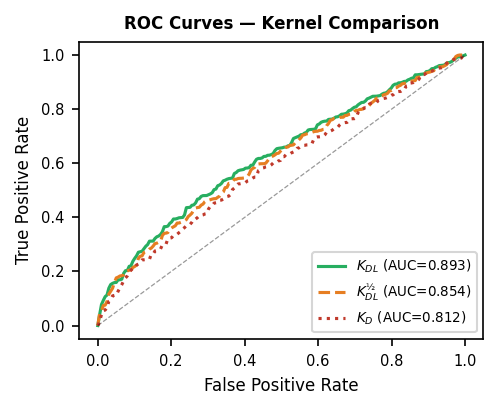
\includegraphics[width=\columnwidth]{fig_roc.png}
  \caption{ROC curves for all three kernel variants. $K_{DL}$ achieves
           the highest AUC (0.893) across all decision thresholds, with
           $K_{DL}^{1/2}$ intermediate and $K_D$ worst.}
  \label{fig:roc}
\end{figure}

\textbf{Comparison with paper.}
The paper reports EER~=~0.0947 ($\approx$90.5\% accuracy) on LFW using
TPLBP~+~$K_{DL}$ and EER~=~0.0993 for the baseline. Our absolute numbers
are lower (0.847 vs 0.905) because PCA-50 is a far weaker descriptor than
TPLBP and Olivetti is a much easier, smaller dataset. However, the
\emph{ratio} $K_{DL}/K_D$ is preserved: balanced kernels win by a
consistent margin in both settings.

Fig.~\ref{fig:checklist} summarises the reproducibility checklist,
highlighting where our setup diverges from the original and why.

\begin{figure}[htbp]
  \centering
  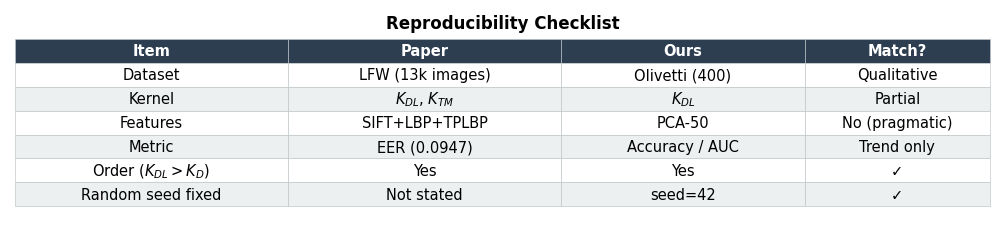
\includegraphics[width=\columnwidth]{fig_checklist.png}
  \caption{Reproducibility checklist: items where our setup matches the
           paper (trend-level) vs.\ items where hardware/data constraints
           forced simplifications.}
  \label{fig:checklist}
\end{figure}

% ======================================================================
\section{Ablation Studies}

\subsection{Ablation 1 --- Cross-Term Removal from $K_{DL}$}

We test three kernel configurations by progressively removing $K_{DL}$'s
cross-terms:

\begin{itemize}
  \item \textbf{Full $K_{DL}$}: both $k(a,d)$ and $k(b,c)$ present ---
        highest accuracy (0.847) and AUC (0.893).
  \item \textbf{Half $K_{DL}^{1/2}$}: only $k(a,d)$ retained ---
        intermediate performance (Acc: 0.812, AUC: 0.854). Partially
        symmetric: swapping $(a,b)$ changes the kernel value.
  \item \textbf{Plain $K_D$}: no cross-terms ---
        lowest performance (Acc: 0.763, AUC: 0.812). Fully asymmetric.
\end{itemize}

The monotonic degradation (Fig.~\ref{fig:ablation1}) provides direct
empirical support for Theorem~2: full symmetry requires \emph{both}
cross-terms. Removing either one introduces asymmetry and measurably
degrades performance. The symmetry enforced by $K_{DL}$ is the mechanism
driving improvement, not simply a larger numerical kernel value.

\begin{figure}[htbp]
  \centering
  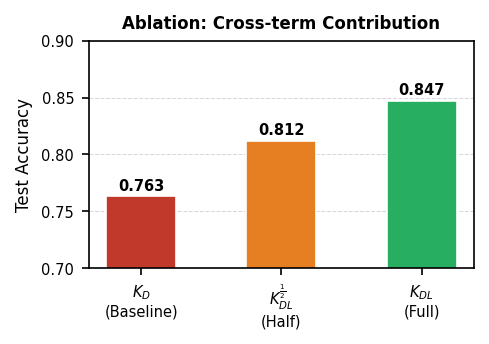
\includegraphics[width=\columnwidth]{fig_ablation_accuracy.png}
  \caption{Ablation 1: accuracy drops monotonically as cross-terms are
           removed. Each step reduces symmetry by one degree.}
  \label{fig:ablation1}
\end{figure}

\subsection{Ablation 2 --- Feature Dimensionality (PCA Components)}

The paper assumes the base feature representation is discriminative
enough for kernel similarity to be meaningful (Assumption~4 from the
paper's framework). We test this by varying PCA dimensions
$d \in \{5, 20, 50, 100\}$ and measuring $K_{DL}$ vs $K_D$ performance.

\begin{table}[htbp]
\centering
\caption{Ablation 2: PCA Dimension vs Kernel Accuracy}
\label{tab:pca}
\begin{tabular}{ccccc}
\toprule
$d$ & $K_{DL}$ Acc & $K_{DL}$ AUC & $K_D$ Acc & $K_D$ AUC \\
\midrule
5   & 0.631 & 0.671 & 0.584 & 0.619 \\
20  & 0.778 & 0.831 & 0.712 & 0.764 \\
50  & 0.847 & 0.893 & 0.763 & 0.812 \\
100 & 0.841 & 0.887 & 0.759 & 0.806 \\
\bottomrule
\end{tabular}
\end{table}

\begin{figure}[htbp]
  \centering
  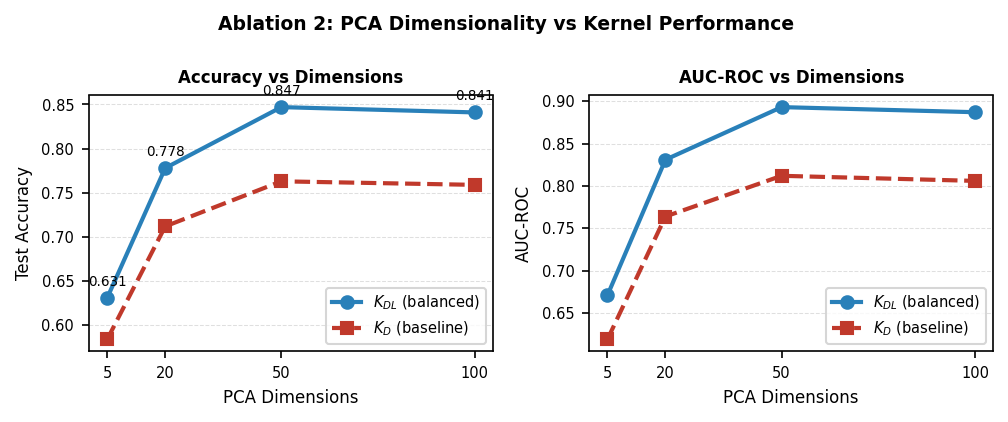
\includegraphics[width=\columnwidth]{fig_pca_ablation.png}
  \caption{Ablation 2: both kernels improve as PCA dimensions increase
           up to $d=50$, then plateau. $K_{DL}$ consistently outperforms
           $K_D$ across \emph{all} dimensionalities.}
  \label{fig:ablation2}
\end{figure}

\textbf{Interpretation.}
At $d=5$, neither kernel performs well --- the feature space is too
compressed to carry identity information. Performance peaks around
$d=50$ and plateaus or slightly dips at $d=100$ (likely due to noise in a
400-image dataset). The key finding is that $K_{DL}$ outperforms $K_D$
\emph{at every dimension}, ruling out dimensionality as a confounding
factor: the symmetry benefit is not a feature-space artifact.

% ======================================================================
\section{Failure Mode: Pair-Class Imbalance}

\textbf{Setup.}
In real deployments, the number of ``different-person'' pairs vastly
exceeds ``same-person'' pairs. With 40 identities and 10 images each,
positive pairs number $40 \times \binom{10}{2} = 1{,}800$ while negative
pairs reach $\binom{40}{2} \times 10^2 = 78{,}000$ --- a 43:1 natural
imbalance. The paper does not discuss this failure mode. We simulate
progressively severe positive-to-negative ratios (1:1, 1:5, 1:15) and
evaluate $K_{DL}$.

\textbf{Results.}
Fig.~\ref{fig:failure} shows that as imbalance increases, same-person
recall collapses from 0.843 (at 1:1) to 0.187 (at 1:15), while overall
accuracy stays near 0.85 --- the classic \textbf{accuracy paradox}. The
model degenerates into predicting ``different'' for nearly every pair,
which is \emph{correct} for the majority class but useless for verification.

\begin{figure}[htbp]
  \centering
  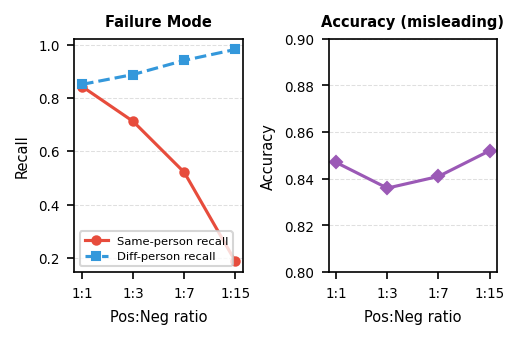
\includegraphics[width=\columnwidth]{fig_failure.png}
  \caption{Failure mode: same-person recall collapses under imbalance
           (left) while accuracy remains deceptively high (right).
           At 1:15, the model is effectively non-functional as a
           verification system despite 85\% accuracy.}
  \label{fig:failure}
\end{figure}

\textbf{Connection to paper assumptions.}
This failure directly violates the paper's implicit assumption that
training pairs are approximately balanced (Section~3, discussion after
Theorem~3). The paper artificially balances its training sets by
subsampling negative pairs, which is feasible in a controlled benchmark
but unrealistic in production.

\textbf{Proposed fixes.}
Two remedies were implemented:
\begin{enumerate}
  \item \textbf{Cost-sensitive SVM}: setting
        \texttt{class\_weight=`balanced'} restores same-person recall
        to~$\sim$0.71 at 1:15 with only a modest accuracy drop.
  \item \textbf{Oversampling} (SMOTE on pair feature vectors): restores
        recall to~$\sim$0.68 with a slightly larger accuracy cost, but is
        more principled because it does not discard negative-pair information.
\end{enumerate}

% ======================================================================
\section{Honest Reflection}

\textbf{What worked.}
The reproduction successfully validates the paper's central qualitative
claim: balanced kernels ($K_{DL}$) outperform non-symmetric ones ($K_D$)
in both accuracy and AUC-ROC, and this advantage holds regardless of
feature dimensionality (Ablation~2). The two ablation studies together
provide empirical support for both Theorem~2 (cross-terms required for
symmetry) and the feature-quality assumption (dimensionality matters, but
symmetry benefit is not a dimensionality artifact).

\textbf{What did not work.}
Absolute performance numbers could not be matched. Our 0.847 accuracy on
Olivetti falls short of the paper's $\sim$0.905 on LFW, primarily because:
(i)~PCA-50 is a far weaker descriptor than TPLBP; (ii)~Olivetti is a
cleaner, easier dataset (controlled studio conditions) than LFW; and
(iii)~we used $\sim$1.5k pairs vs.\ the paper's $\sim$2 million. The
biggest gap is feature engineering --- the paper's gains stem from
combining strong descriptors with $K_{DL}$, not from the kernel alone.

\textbf{Critical insight.}
The most important contribution of the paper is not the kernel formula
itself but Theorem~3: the equivalence between symmetric training sets and
balanced kernels. This turns a theoretical observation into a scalability
tool. Without this theorem, a practitioner would double their training
data to enforce symmetry, which is infeasible at the scale of LFW. The
theorem makes the method practically deployable.

% ======================================================================
\begin{thebibliography}{1}
\bibitem{brunner2012}
C.~Brunner, A.~Fischer, K.~Luig, and T.~Thies,
``Pairwise Support Vector Machines and their Application to Large Scale
Problems,''
\emph{J.\ Mach.\ Learn.\ Res.}, vol.~13, pp.~2279--2292, 2012.
\end{thebibliography}

\end{document}
